%openany impede que sejam feitas paginas em branco após o fim do capítulo
\documentclass[openany,10pt,a4paper]{book}
\usepackage[utf8]{inputenc}
\usepackage[portuguese]{babel}
\usepackage[T1]{fontenc}
\usepackage{amsmath}
\usepackage{amsfonts}
\usepackage{amssymb}
\usepackage{makeidx}
\usepackage{graphicx}
\usepackage{setspace}
\usepackage{indentfirst}
\usepackage[Conny]{fncychap}
\usepackage[left=2cm,right=2cm,top=2cm,bottom=2cm]{geometry}
\author{Charles Hernique Porto Ferreira}
\title{Manual do Desenvolvedor}

\begin{document}
%\maketitle

%************************************************************************************************
														%Capa
%************************************************************************************************
\clearpage
%% temporary titles
% command to provide stretchy vertical space in proportion
\newcommand\nbvspace[1][3]{\vspace*{\stretch{#1}}}
% allow some slack to avoid under/overfull boxes
\newcommand\nbstretchyspace{\spaceskip0.5em plus 0.25em minus 0.25em}
% To improve spacing on titlepages
\newcommand{\nbtitlestretch}{\spaceskip0.6em}
\pagestyle{empty}
\begin{center}
\bfseries
\nbvspace[1]
\Huge
{\nbtitlestretch\huge
RESERVAS DE SALAS E EQUIPAMENTOS UFABC}

\nbvspace[1]
\normalsize

\Large MANUAL DO USUÁRIO\\
%LINERS AND CODE SO THAT\\
%YOU CAN AWK LIKE A HAWK
\nbvspace[1]
\small desenvolvimento:\\
\normalsize CHARLES HENRIQUE PORTO FERREIRA\\[0.5em]
\small supervisão:\\
\normalsize ANDRÉ GUILHERME RIBEIRO BALAN\\[0.5em]
%\footnotesize AUTHOR OF ``A WORKING ALGEBRA,'' ``WIRELESS TELEGRAPHY,\\
%ITS HISTORY, THEORY AND PRACTICE,'' ETC., ETC.

\nbvspace[2]

%\includegraphics[width=1.5in]{./graphics/pic37}
\nbvspace[3]
\normalsize

UFABC\\
\large
UNIVERSIDADE FEDERAL DO ABC\\
\normalsize
CMCC\\
\large
CENTRO DE MATEMÁTICA, COMPUTAÇÃO E COGNIÇÃO
\nbvspace[1]
\end{center}
%************************************************************************************************
\onehalfspace
\tableofcontents

\chapter{Introdução}
Este manual explica todas as funções presentes no Aplicativo \textit{Reservas de Salas UFABC}. No geral o aplicativo é bem simples contendo funções simples que atendam as necessidades da divisão acadêmica do Centro de Matemática, Computação e Cognição (CMCC) da Universidade Federal do ABC (UFABC). Inicialmente o aplicativo foi desenvolvido para substituir o antigo sistema que feito usando o Google Calendar, o qual não gerenciava problemas de reservas feitas no mesmo horário. Durante o desenvolvimento do aplicativo novas funcionalidades foram sendo adicionadas conforme as necessidades dos funcionários do CMCC.


\chapter{Instalação}
O aplicativo ``roda'' na \textit{Web} logo não é necessária a instalação\footnote{Detalhes de como colocar o aplicativo na \textit{web} podem ser encontrado no Manual do Desenvolvedor.}.\\ O link para acessá-lo é: \textbf{\textit{http://reservas.cmcc.ufabc.edu.br/}}

\chapter{Funções}
O aplicativo oferece funções para reservar salas e equipamentos. Todas elas são explicadas abaixo

\section{Login}
O aplicativo oferece um sistema de login integrado ao sistema da UFABC. Para acessá-lo, é necessário colocar seu nome de usuário e senha utilizados nos sistemas da UFABC (tidia, e-mail, biblioteca, entre outros). Apesar de ser integrado ao usuário da UFABC, o login garante que apenas usuários autorizados e cadastrados no Sistema de Reservas de sala possam utilizá-lo, servindo como uma segurança para o aplicativo.

\begin{figure}[!htb]
    \centering
    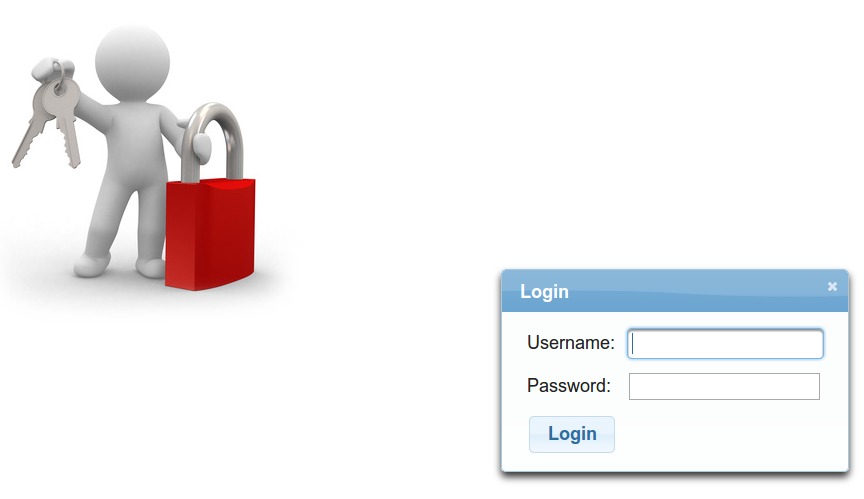
\includegraphics[scale=0.4]{login.png}
    \caption{Tela de login}
    \label{im_Login}
\end{figure}

Ao clicar na imagem será mostrado uma janela requisitando o login conforme Figura \ref{im_Login}. Insira o login e clique no botão Login. Após a autenticação, deverá ser mostrado o Calendário de reservas, Figura \ref{im_calendario}.
 
 \begin{figure}[!htb]
     \centering
     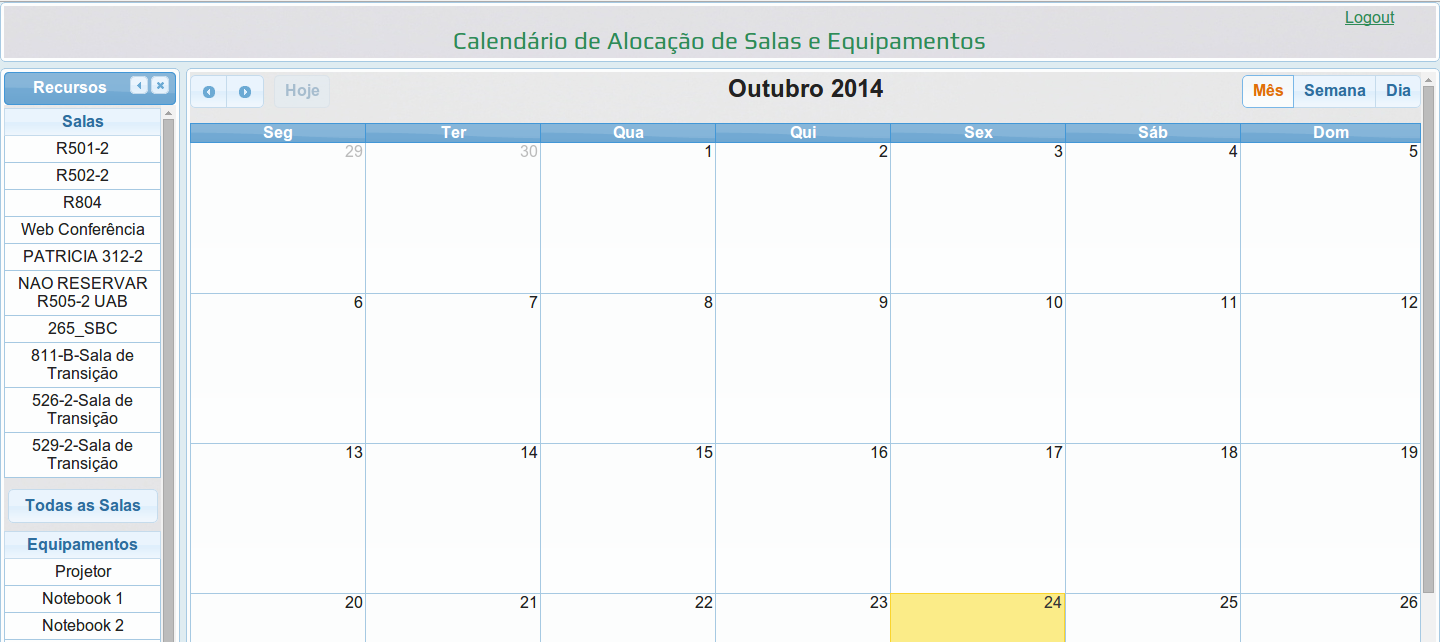
\includegraphics[scale=0.3]{calendario.png}
     \caption{Calendário de reservas}
     \label{im_calendario}
 \end{figure}




\section{Cadastrar, Remover e Atualizar}

A primeira vez que o aplicativo é instalado, sua base de dados está vazia sendo necessário criar as \textbf{salas}, \textbf{equipamentos}, \textbf{docentes}, \textbf{TAs} e \textbf{usuários} para gerenciar as reservas.
Todo o gerenciamento destes dados pode ser feito na tela Gerenciar Dados, que aparece ao clicar no botão \textbf{Gerenciar Dados}, na tela do Calendário.

A Figura \ref{im_gerenciarDados} mostra as opções disponíveis.

\begin{enumerate}
\item{\textbf{Centros}}\\
Permite cadastrar, alterar e excluir centros.
\item{\textbf{Docente}}\\
Permite cadastrar, alterar e excluir docente.s
\item{\textbf{TA}}\\
Permite cadastrar, alterar e excluir Técnicos Administrativos (TAs).
\item{\textbf{Salas}}\\
Permite cadastrar, alterar e excluir salas.
\item{\textbf{Equipamentos}}\\
Permite cadastrar, alterar e excluir equipamento.
\item{\textbf{Calendário}}\\
Mostra o calendário.
\item{\textbf{Empréstimo}}\\
Permite alterar e excluir empréstimos.
\item{\textbf{Usuários}}\\
Permite cadastrar, alterar e excluir usuários do Sistema de Reservas. Essa função é restrita aos usuários administradores do sistema. 
\end{enumerate}

\begin{figure}[!htb]
     \centering
     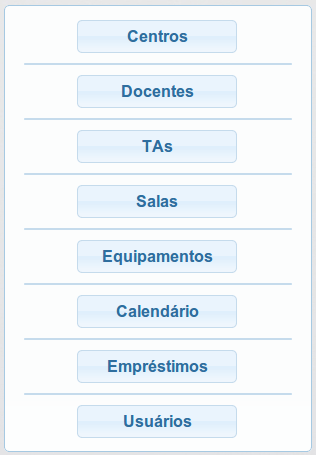
\includegraphics[scale=0.4]{gerenciarDados.png}
     \caption{Tela Gerenciar Dados}
     \label{im_gerenciarDados}
 \end{figure} 


As três tarefas do gerenciamento de dados (criar, alterar e excluir) do Centro, Docente, TA, Salas e Equipamentos são bem similares para todos eles. Segue um exemplo do gerenciamento com docente.

\begin{enumerate}
\item{Criar docente}\\
Ao clicar no botão Docente o browser será redirecionado para a tela de gerenciamento de docentes. Esta tela contém uma lista de todos os docentes já cadastrados, Figura \ref{im_listaDocentes}, caso haja algum. Descendo a barra de rolagem, aparece a área destinada a criação dos docentes. Existem quatro campos que devem ser preenchidos, como mostra a Figura \ref{im_criarDocente}\footnote{Para inserir o centro é necessário criá-lo antes.}\footnote{O número de matrícula deve ser único para cada docente.}. 

\begin{figure}[!htb]
    \centering
    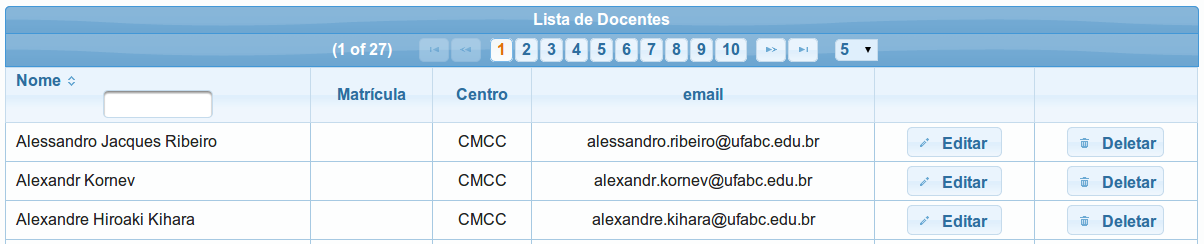
\includegraphics[scale=0.32]{listaDocentes.png}
    \caption{Lista de docentes}
    \label{im_listaDocentes}
\end{figure}

\begin{figure}[!htb]
    \centering
    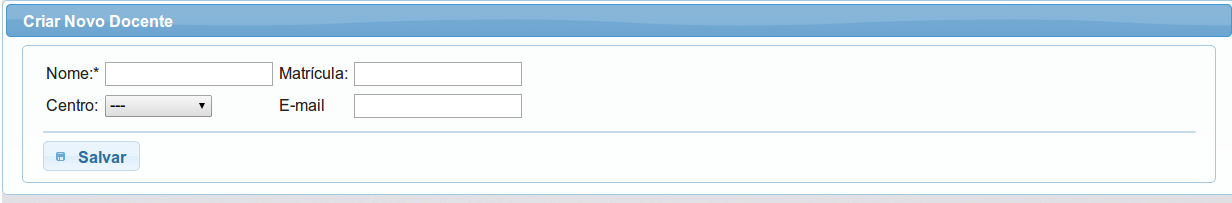
\includegraphics[scale=0.3]{criarDocente.png}
    \caption{Área para criação de docentes}
    \label{im_criarDocente}
\end{figure}


\item{Alterar docente}\\
Para alterar os dados do docente, clique no botão \textit{Editar} da lista. Será aberta a tela da Figura \ref{im_editarDocente} com os dados do docente selecionado. Clicando no link \textit{Atualizar Docente} os dados são atualizados no banco de dados.

\begin{figure}[!htb]
    \centering
    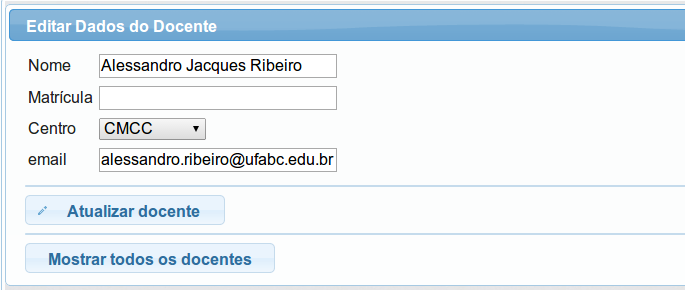
\includegraphics[scale=0.4]{editarDocente.png}
    \caption{Área para edição de docente}
    \label{im_editarDocente}
\end{figure}
\item{Excluir docente}\\
para remover o docente clique no link \textit{Deletar} na lista de docentes.
\end{enumerate}


\section{Reservas}

Nas próximas seções será explicada detalhadamente a principal função desse sistema. 

\subsection{Criar Reserva}

Com os docentes, salas e/ou equipamentos cadastrados é possível fazer as reservas. Na tela do calendário, selecione a sala ou equipamento que deseja reservar. Após o clique deverá ser mostrado todas as reservas referentes à escolha feita, isto é, caso haja alguma reserva feita.\\
Clique no dia que deseja fazer a reserva que será aberta uma janela com os informações necessárias como mostra a Figura \ref{im_criarReserva} .

\begin{figure}[!htb]
    \centering
    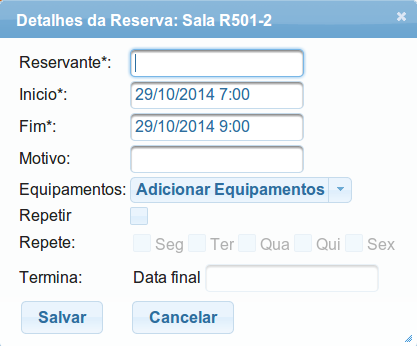
\includegraphics[scale=0.5]{criarReserva.png}
    \caption{Área de criação de Reservas}
    \label{im_criarReserva}
\end{figure}


\begin{enumerate}
\item{Reservante}\\
No campo Reservante digite o nome do docente que deseja reservar a sala. Conforme forem digitadas as primeiras letras será mostrado o nome dos reservantes cadastrados, selecione o nome que deseja quando aparecer.
\item{Início}\\
Este campo permite selecionar a hora de início da reserva. A hora deve ser configurada deslizando a barra de rolagem que encontra-se na parte inferior da janela que é aberta, Figura \ref{im_inicio}.

\begin{figure}[!htb]
    \centering
    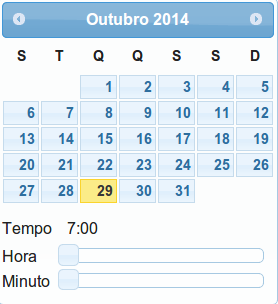
\includegraphics[scale=0.5]{inicio.png}
    \caption{Área para configuração do início da reserva}
    \label{im_inicio}
\end{figure}
\item{Fim}\\
Este campo permite selecionar a hora de início da reserva. A hora deve ser configurada deslizando a barra de rolagem que encontra-se na parte inferior da janela que é aberta, Figura \ref{im_fim}.

\begin{figure}[!htb]
    \centering
    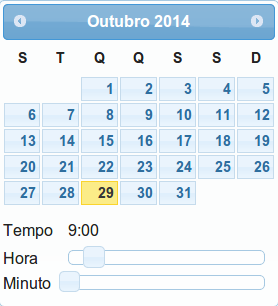
\includegraphics[scale=0.5]{fim.png}
    \caption{Área para configuração do fim da reserva}
    \label{im_fim}
\end{figure}
\item{Motivo}\\
O motivo é um campo opcional que permite armazenar o motivo da reserva, caso este seja especificado.
\item{Adicionar Equipamentos}\\
Este campo permite que sejam reservados equipamentos junto com a sala.
\item{Repetir}\\
Ao selecionar este \textit{checkbox} será liberada a opção de criar reservas semanais.
\item{Repete}\\
Se o \textit{checkbox} ``Repetir'' for selecionado esta opção é liberada e permite escolher os dias da semana que serão repetidas as reservas.
\item{Termina}\\
Caso o \textit{checkbox} ``Repetir'' estiver selecionado este campo permite selecionar a data final da reserva semanal.
\end{enumerate}

Os três primeiros campos são obrigatórios para criação das reservas. Após preenche-los clique no botão ``Salvar'' para armazenar os dados no banco de dados \footnote{Quando uma reserva é feita, o reservante recebe um email com os dados da reserva.}.
\subsection{Editar Reserva}
Ao selecionar a reserva feita é aberta uma janela que permite editar os dados da reserva. Após a alteração dos dados, clique no botão ``Atualizar'' para gravar os dados no banco de dados.

\subsection{Remover Reserva}
Selecione, no calendário, uma reserva já feita que será aberta a opção de edição de dados da reserva. Clique no botão ``Remover'' para apagar a reserva.

\subsection{Criar várias reservas}
O sistema permite que sejam feitas várias reservas ao mesmo tempo para o mesmo reservante, especificando os dias da semana que serão feitas as reservas e a data final da reserva, como na Figura \ref{im_variasReservas}.

\begin{figure}[!htb]
    \centering
    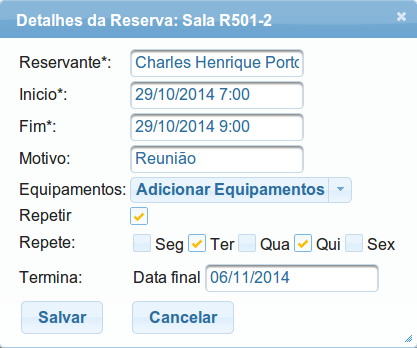
\includegraphics[scale=0.5]{variasReservas.png}
    \caption{Exemplo de criação de várias reservas}
    \label{im_variasReservas}
\end{figure}

\section{Empréstimo}

Após a reserva ser feita o reservante deverá retirar a chave da sala ou o equipamento que reservou. Neste momento é preciso registrar o item que esta sendo levado pelo reservante, através da criação de um Empréstimo.

\subsection{Criar Empréstimo}

 Clique na reserva feita para que seja aberta a janela de edição da reserva onde deve aparecer a opção de ``Criar Empréstimo'', Figura \ref{im_criarEmprestimo}.

\begin{figure}[!htb]
    \centering
    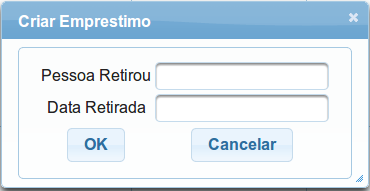
\includegraphics[scale=0.45]{criarEmprestimo.png}
    \caption{Área para criação de empréstimo}
    \label{im_criarEmprestimo}
\end{figure}

\begin{enumerate}
\item{Pessoa Retirou}\\
Digite o nome da pessoa que retirou a chave da sala e/ou o equipamento.
\item{Data Retirada}\\
Selecione a data e hora que foi feita a retirada. Ao clicar no botão ``Hoje'' será puxado a hora atual do sistema.
\end{enumerate}

\subsection{Finalizar Empréstimo}
Quando um empréstimo é criado é  mostrado uma lista contendo todos os empréstimos. Esta lista também pode ser acessada pela tela Gerenciar Dados, acessando o botão Empréstimo.\\
Quando o reservante vem devolver a chave da sala e/ou equipamento reservado e necessário acessar essa lista, clicar no link Editar, para poder registrar a hora da devolução e a pessoa responsável pela recepção do(s) item(s).


\section{Email}
Toda vez que uma reserva é criada, um empréstimo é feito e um empréstimo é finalizado, o reservante recebe um email de notificação automaticamente.


\section{Mostrar todas as reservas}
Na tela do calendário existe um botão chamado ``Todas as salas''. Ao clicar nele, são mostradas todas as reservas das salas ao mesmo tempo. Essa visualização permite que se tenha um visão geral de todas as salas reservas porém não permite editar as reservas feitas. Para poder editá-las é necessário selecionar a sala, lado esquerdo, que se deseja editar, onde será  mostrado todas as reservas daquela sala em específico.

\section{Mostrar todos os equipamentos}
Assim como o botão para mostrar todas as salas reservadas simultaneamente, há um botão ``Todos Equipamentos'', que mostra todas as reservas de equipamentos do mês que está sendo visualizado. Da mesma forma, não é possível editar as reservas feitas, é necessário clicar no equipamento que se deseja editar na barra lateral esquerda. 

\section{Usuários}
Para utilizar o sistema, não é suficiente apenas inserir o login e a senha utilizados na UFABC, também é necessário ser um usuário cadastrado no sistema. O sistema já possuirá um usuário inicial cadastrado, para que o login possa ser efetuado na primeira vez que o aplicativo for utilizado. Esse usuário será um usuário administrador, o que significa que ele tem permissão para cadastrar, editar e excluir outros usuários. Usuários que não são administradores não terão acesso à página de gerência de dados de usuários, mas terão acesso a todas as outras funcionalidades do Sistema de Reservas. 

\subsection{Cadastrar um Usuário}

Caso o usuário seja um administrador do sistema, ele poderá cadastrar outros usuários, clicando em ``Usuários'' na tela de gerenciamento de dados. Depois, na área mostrada na Figura \ref{criarUsuario}, deve escolher o nome do TA (previamente cadastrado) que será um usuário do sistema e clicar na caixa ``Usuário Administrador'', caso aquele novo usuário deva ser um administrador também. 

\begin{figure}[!htb]
    \centering
    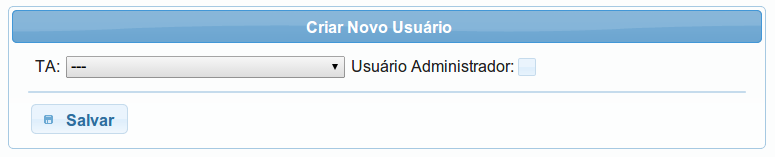
\includegraphics[scale=0.5]{criarUsuario.png}
    \caption{Área para criação de um usuário}
    \label{criarUsuario}
\end{figure}

O sistema utiliza o nome do TA para acessar o nome de usuário do sistema de logins da UFABC. Caso o TA não tenha sido registrado com o mesmo nome presente no sistema da UFABC, o aplicativo de reservas não conseguirá ter acesso a esse login, e vai requisitar que o login seja inserido manualmente (esse login também deve ser o mesmo que é utilizado nos sistemas da UFABC). A Figura \ref{wanessa} ilustra a tentativa de cadastro de um usuário para a TA Wanessa. Porém, como o nome dela não foi registrado por completo, ocorrerá um erro no sistema e ele irá solicitar o preenchimento manual do login, como mostra a Figura \ref{erroUsuario}.

\begin{figure}[!htb]
    \centering
    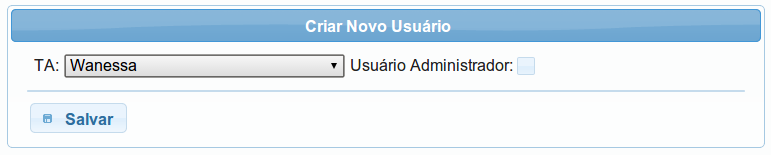
\includegraphics[scale=0.5]{wanessa.png}
    \caption{Tentativa de criação de um usuário}
    \label{wanessa}
\end{figure}

\begin{figure}[!htb]
    \centering
    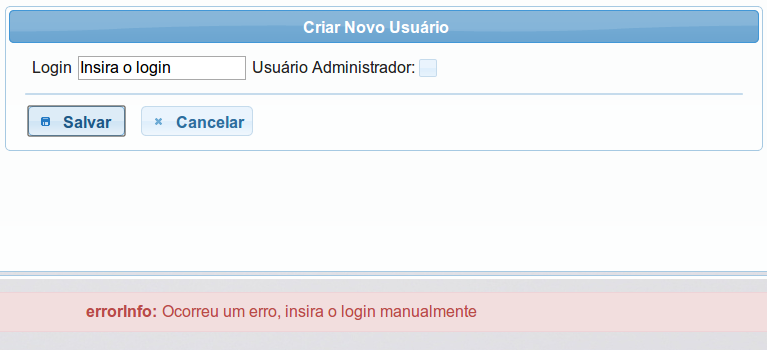
\includegraphics[scale=0.5]{erroUsuario.png}
    \caption{Erro na criação de um usuário}
    \label{erroUsuario}
\end{figure}

O usuário deve então inserir o login correto (``Insira o login'') e clicar em (``Salvar'') para cadastrar o usuário, como mostra a Figura \ref{loginWanessa}. Caso não queira cadastrar um usuário para o TA escolhido anteriormente, basta clicar em ``Cancelar''.

\begin{figure}[!htb]
    \centering
    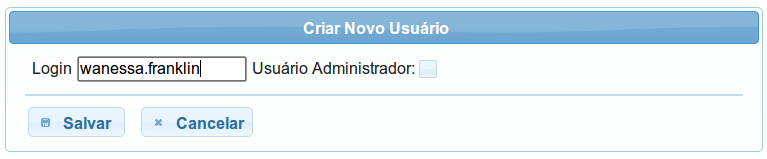
\includegraphics[scale=0.5]{loginWanessa.png}
    \caption{Inserção manual do login}
    \label{loginWanessa}
\end{figure}

O usuário será salvo e ficará disponível para ser editado ou apagado na lista de usuários, Figura \ref{listaUsuarios}.

\begin{figure}[!htb]
    \centering
    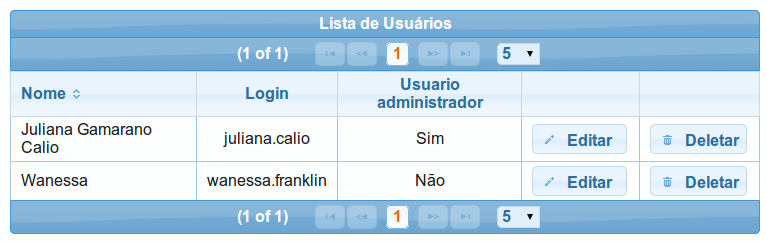
\includegraphics[scale=0.5]{listaUsuarios.png}
    \caption{Lista de Usuários}
    \label{listaUsuarios}
\end{figure}

\subsection{Editar um usuário}

Caso o login tenha sido inserido incorretamente no cadastro de um usuário, é possível editá-lo, clicando em ``Editar'' na lista de usuários. Além disso, é possível tornar um usuário administrador ou remover essa propriedade através da edição, Figura \ref{editarUsuario}.

\begin{figure}[!htb]
    \centering
    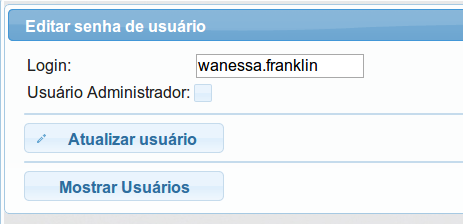
\includegraphics[scale=0.5]{editarUsuario.png}
    \caption{Tela de edição de usuário}
    \label{editarUsuario}
\end{figure}

\subsection{Deletar um usuário}
Para deletar um usuário, basta clicar em ``Deletar'' na lista de usuários.

\section{Logout}
Para realizar sair do sistema, clique em ``Logout'' no canto superior direito da tela, como na Figura \ref{logout}.

\begin{figure}[!htb]
    \centering
    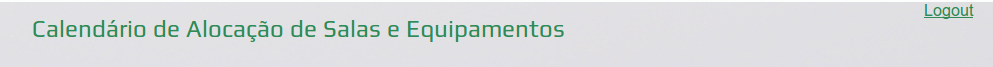
\includegraphics[scale=0.5]{logout.png}
    \caption{Logout do sistema}
    \label{logout}
\end{figure}

\chapter{Validações}

Para a maioria dos erros que ocorrem durante a execução do programa existe uma mensagem com o motivo do erro. Em alguns casos será necessário uma intervenção do usuário.

\section{Tela congelada}
Ao fazer o login, o sistema é liberado para uso. Se o \textit{browser} ficar muito tempo ``parado'', ou seja, sem nenhuma ação executada pelo usuário, o calendário não responderá mais sendo necessário fazer o login novamente. Se acontecer uma situação semelhante, atualize o \textit{browser} (geralmente o botão F5 do teclado) para ser redirecionado à tela de login.
Essa é uma medida de segurança para que outros usuários não acessem o sistema indevidamente que alguém deixou logado.

\section{Reserva feita no mesmo horário}
O sistema verifica se alguma reserva é feita na mesma data/hora e impede que isso aconteça. Uma mensagem de erro aparece na tela informando sobre o ocorrido, Figura \ref{im_reservaOcupada}. 

\begin{figure}[!htb]
    \centering
    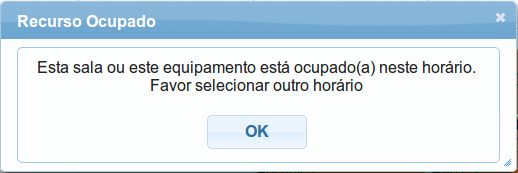
\includegraphics[scale=0.4]{reservaOcupada.png}
    \caption{Mensagem de erro ao tentar fazer uma reserva em um horário já reservado}
    \label{im_reservaOcupada}
\end{figure}


\section{Não selecionar uma sala ou equipamento para reservar e clicar na data}
Logo após o login, o sistema abre o calendário porém nenhum item foi selecionado para fazer reserva ainda. Caso o usuário clique em alguma data para para fazer a reserva sem antes especificar ``o que'' ele quer reservar, será mostrada uma mensagem na tela informando que ele deve selecionar alguma sala ou equipamento, Figura \ref{im_selecioneSalaEquipamento}.

\begin{figure}[!htb]
    \centering
    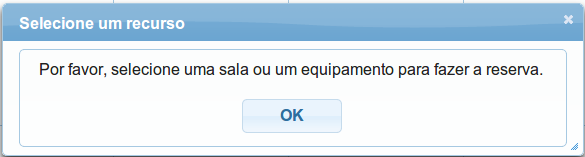
\includegraphics[scale=0.4]{selecioneSalaEquipamento.png}
    \caption{Mensagem informando que deve ser selecionado a sala ou o equipamento que se deseja reservar}
    \label{im_selecioneSalaEquipamento}
\end{figure}

\section{Selecionar uma data que já expirou}

O sistema bloqueia reservas feitas em datas anteriores ao dia atual. Uma mensagem informando o ocorrido aparece na tela caso isso ocorra, Figura \ref{im_dataExpirou}.

\begin{figure}[!htb]
    \centering
    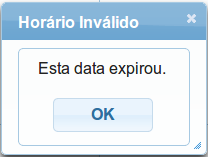
\includegraphics[scale=0.45]{dataExpirou.png}
    \caption{Mensagem data expirou}
    \label{im_dataExpirou}
\end{figure}

\section{Erro ao criar um novo docente ou técnico administrativo}
Todo docente e técnico administrativo possuem um número de identificação único, a matrícula. Caso esse número seja igual ao de outro docente/TA, o sistema não permitirá o cadastro ou atualização do cadastro. \\
O mesmo pode


\chapter{Contato}
\centering 
Centro de Matemática, Computação e Cognição (CMCC)\\
Universidade Federal do ABC (UFABC)\\





\end{document}